\documentclass{report}
\usepackage[utf8]{inputenc}
\usepackage[francais]{babel}
\usepackage[T1]{fontenc}
\usepackage{lmodern}
\usepackage{ifpdf}
\usepackage{graphicx}
\usepackage{geometry}
\renewcommand{\familydefault}{\sfdefault}

\geometry{hmargin=50pt, vmargin=50pt}

\title{Rapport de projet : Tableau virtuel interactif}
\author{Baptiste Saleil \and Geoffrey Mélia \and Julien Pagès \and Kevin Bollini}
\date{\today}
\ifpdf
	\pdfinfo 
	{
		/Author (bsaleil,gmelia,jpages,kbollini)
		/Title (Rapport de projet)
		/Subject (Tableau virtuel interactif)
		/Keywords ()
		/CreationDate (\today)
	}
\fi

\begin{document}
	% Page de titre
	\maketitle
	\thispagestyle{empty}
	\newpage
	
	% Sommaire
	\tableofcontents

	%Table des figures
	\listoffigures
	
	\newpage
	\chapter{Introduction}
		\section{Présentation}
		Le but principal du projet est de simuler une écriture ou un dessin sur un tableau virtuel interactif. \\
		Pour cela nous utiliserons une interface basée sur la reconnaissance de mouvements.
		
		\section{Contexte}
		% TODO
	
	\chapter{Analyse et conception}
		\section{Étude de l'existant et faisabilité}
		\subsubsection{Faisabilité}
		Notre groupe ayant lui-même proposé ce sujet, celui-ci s'accorde parfaitement à nos formations et spécialités. Le choix de ce sujet a donc été réalisé en fonction de nos expériences, savoir-faire et affinités.\\
Ce projet s'inscrivant dans le cadre d'un TER de notre formation, l'étude de la faisabilité n'incluera pas certains critères comme l'étude de marché, le contexte économique ou le besoin réel. 
Nous allons nous concentrer notamment sur les compétences techniques et de gestion. Pour les parties financement et analyse des coûts, il va sans dire que nous ne disposons d'aucun financement et n'allons utiliser que des outils gratuits. \\
Le projet sera décomposé en deux parties majeures que sont la bibliothèque de suivi et l'application de dessin virtuel (dont les contenus seront détaillés dans des sections qui leur sont propres).
			\paragraph{Application :\\}
L'application doit exploiter le plus efficacement possible la librairie de reconnaissance. Nous voulons donc mettre en place un étalonnage de l'objet à suivre le plus précisément possible. Le projet doit ensuite être exploitable et utile, nous devons donc mettre en place un certain nombre d'outils tels que la possibilité de gommer, changer de forme, de couleur etc. 
Un module réseau est aussi prévu pour une utilisation concurrente et synchronisée. Et bien sûr la fonctionnalité clé de l'application est le tableau virtuel, qui devra donc être exploitable et le dessin devra être fidèle aux mouvements reconnus.
		\subsubsection{Existant}
		La vision par ordinateur et particulièrement le suivi d'objets, sont des domaines connus et pour lesquels il existe de nombreux travaux. Nous pouvons nous inspirer de certains de ces travaux afin de proposer des fonctionnalités plus pertinentes, éviter certains écueuils ou plus directement utiliser des outils existants comme la librairie OpenCV.\\
			\begin{itemize}
				% TODO : détailler un peu plus l'existant
				\item Exemples dans le jeux vidéo : Kinect, Eye-toy, CamSpace (techniques pour l'IHM, par exemple, mouvements continus ou immobilité sur une zone).
				\item Exemples issus de thèses et de projets de recherche (techniques de programmations).
			\end{itemize}
		\section{Gestion du projet}
			\subsection{Choix stratégiques}
			Pour mener à bien ce projet nous avons décidés de découper les tâches en deux sous-parties. \\
			La première sera une bibliothèque de suivi d'objets, et la deuxième partie une application qui utilisera
			cette bibliothèque pour réaliser un logiciel de dessin interactif. \\
			Ce choix présente plusieurs interêts : \\
			\begin{itemize}
				\item{Premièrement, ce découpage permet de bien différencier les tâches, le développement de la librairie requiert des connaissances en traitement d'images pour tracer des couleurs/objets, appliquer des filtres, manipuler les images, etc. Ceci correspond parfaitement à la formation de deux membres du groupe. (Formation IMAGINA Université Montpellier 2). 
				Le développement de l'application, lui, requiert des connaissances en génie logiciel, pour l'architecture de l'application, en IHM, pour la réalisation de l'interface (logicielle et gestuelle), ou encore en réseau pour la mise en place de l'architecture client/serveur. 
				Ces différents points correspondent également parfaitement à la formation des deux autres membres du groupe. (Formation AIGLE Université Montpellier 2). Ainsi, les tâches peuvent bien se répartir en fonction des connaissances et spécialités de chacun.} \\
				\item{Deuxièmement, l'intérêt de ce découpage est d'avoir deux projets complètement indépendants. En effet, la librairie sera développée d'un côté et permettra d'offrir un bon nombre de fonctionnalités de suivis. 
				L'application, elle, se chargera d'utiliser les fonctionnalités de traitement d'image de la librairie en ajoutant une interface graphique, une couche réseau, une connexion aux webcams, la récupération des images etc.
				La librairie et l'application sont donc deux projets développés en parallèles et très modulaires, notre application peut très bien utiliser une autre librairie de traitement d'images, et la librairie peut très bien être utilisée par d'autres application qui offriraient des fonctionnalités totalement différentes de la nôtre.}
			\end{itemize}
			\newpage
			\subsection{Diagramme de Gantt}
				\begin{figure}[!h]
						\centering
						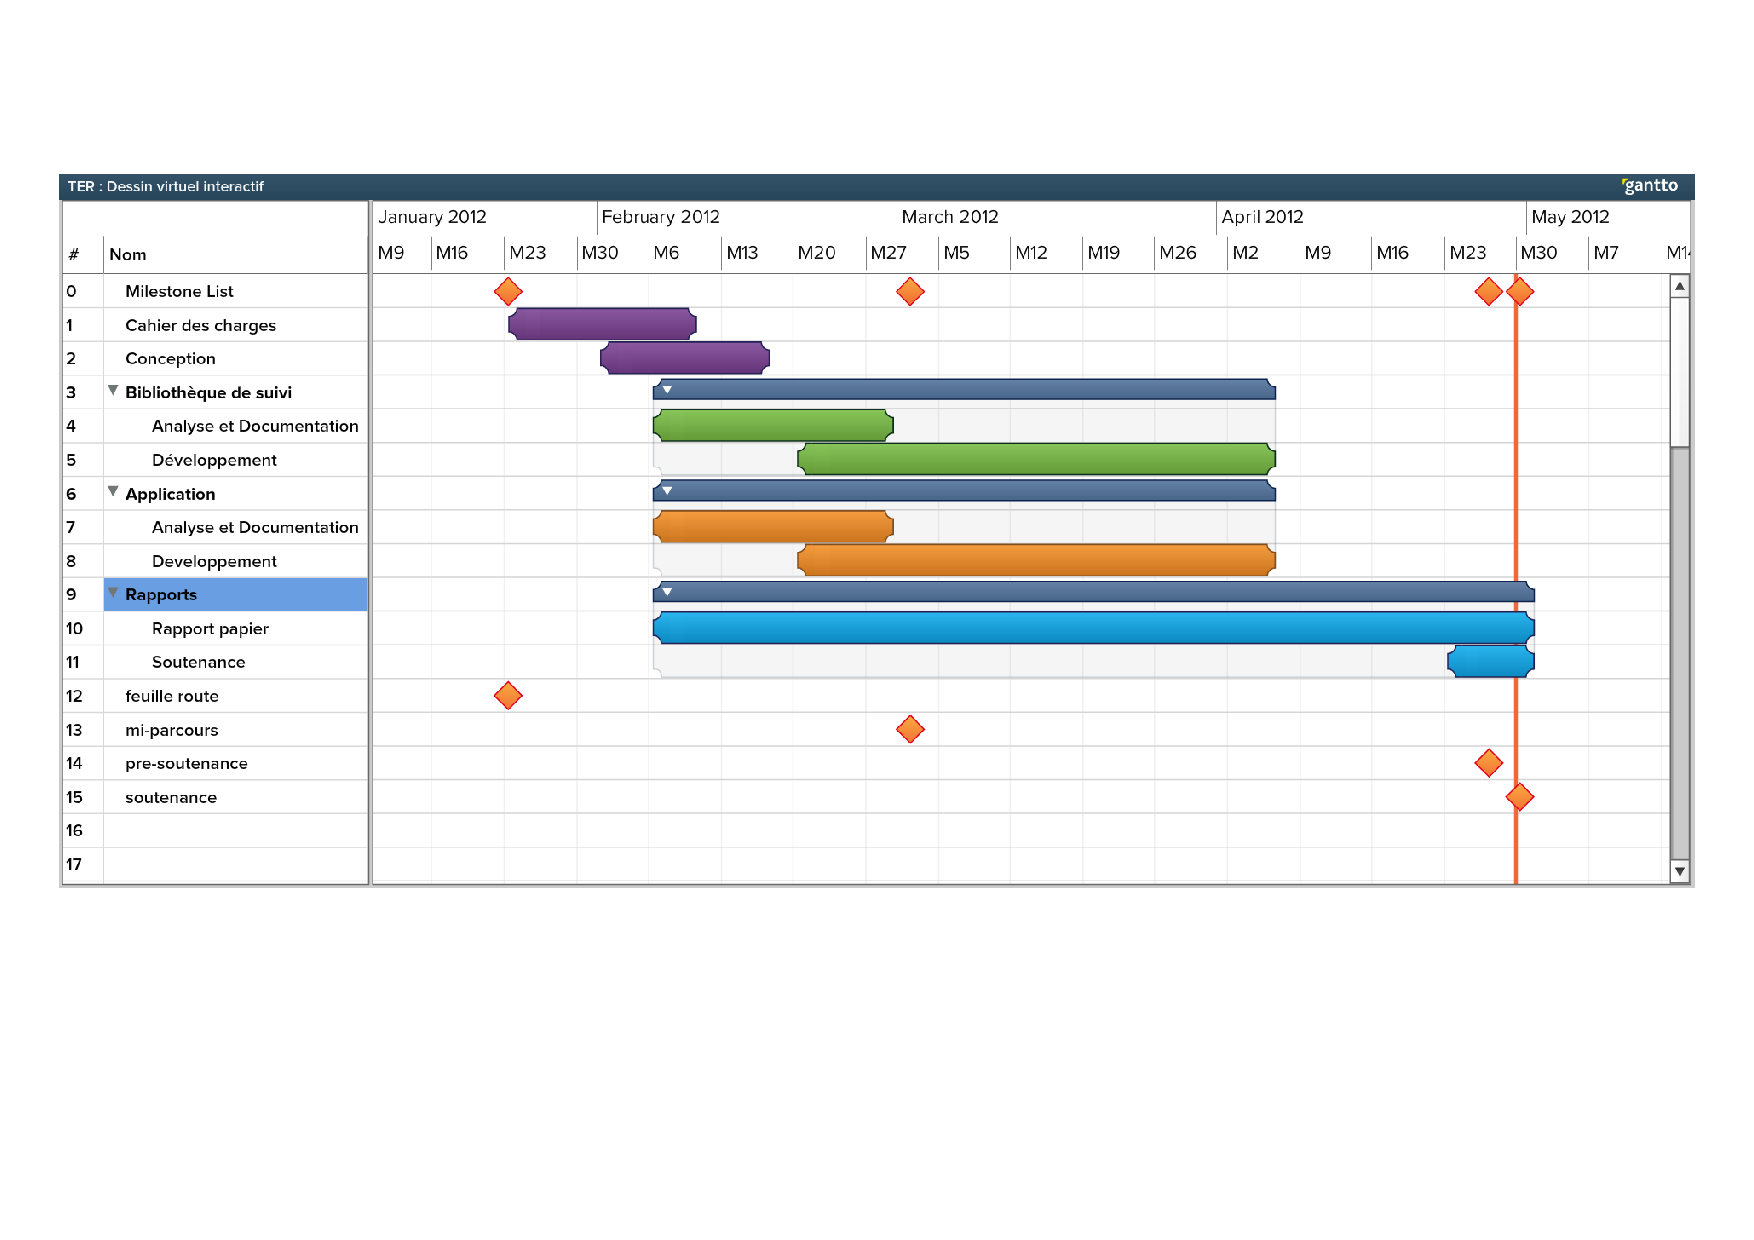
\includegraphics[scale=0.6]{../soutenance/retro-planning.pdf}\\
						\caption{Retroplanning}
						\label{Retroplanning}
				\end{figure}
		\newpage
		\section{Outils utilisés}

		\newpage
		\section{Analyse}
			\subsection{Cas d'utilisations}
				\begin{figure}[!h]
						\centering
						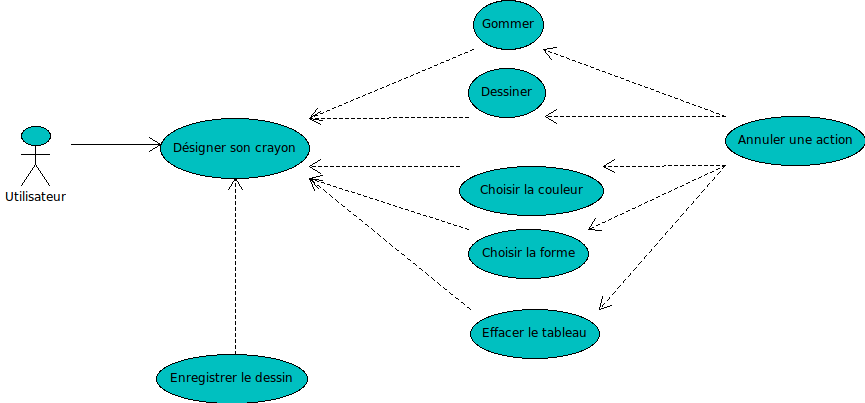
\includegraphics[scale=0.6]{../uml/Dessin.png}\\
						\caption{Cas d'utilisation dessin}
						\label{Cas d'utilisation}
				\end{figure}
			\newpage
			\subsection{Diagrammes de séquences}
				\begin{figure}[!h]
						\centering
						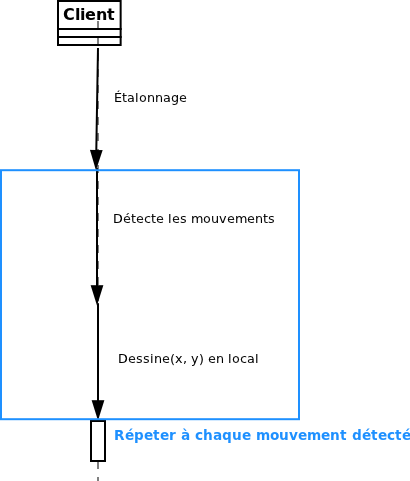
\includegraphics[scale=0.6]{../soutenance/sequence_local.png}\\
						\caption{Diagramme de séquence local}
						\label{Diagramme de séquence local}
				\end{figure}

				\newpage
				\begin{figure}[!h]
						\centering
						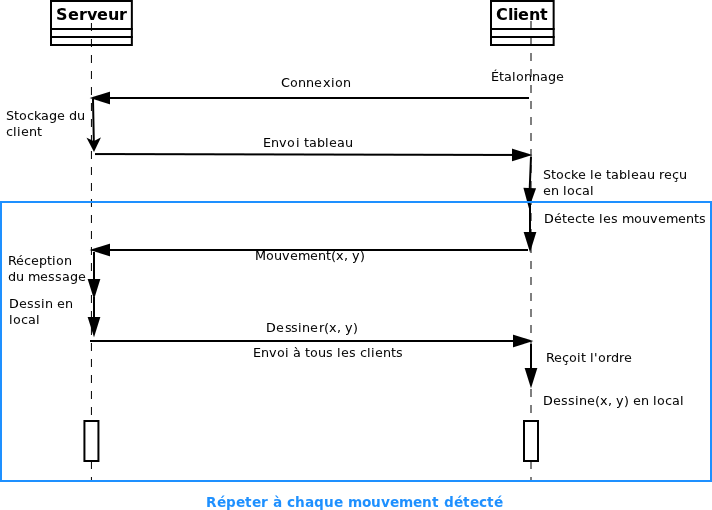
\includegraphics[scale=0.6]{../soutenance/sequence_reseau.png}\\
						\caption{Diagramme de séquence réseau}
						\label{Diagramme de séquence réseau}
				\end{figure}

			\newpage
			\subsection{Diagramme de classes}
				La bibliothèque fonctionne grâce à deux choses, une structure de données et deux fonctions enveloppe. \\
				Le curseur est représenté en mémoire sous la forme d'une strucure de données "Cursor". \\
				Cette structure de données est engendrée par la fonction "calibration" de la librairie, et est utilisée par la suite par l'autre fonction, la fonction "track", qui permet la mise à jour des informations relatives au curseur par rapport à une image. \\
				\begin{figure}[!h]
						\centering
						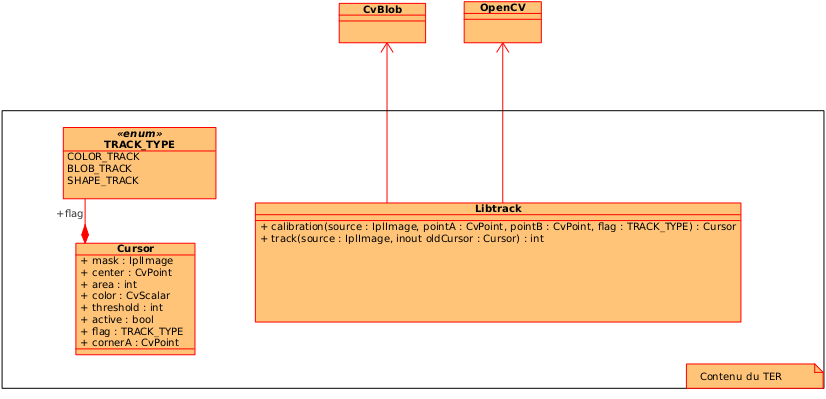
\includegraphics[scale=0.8]{../soutenance/libtrack-uml.png}\\
						\caption{Architrecture de la bibliothèque}
						\label{Architrecture de la bibliothèque}
				\end{figure}

				La bibliothèque dépend de deux bibliothèques externes:
				\begin{itemize}
					\item OpenCV, Spécialisée dans le traitement des images
					\item CvBlob, librairie issue d'OpenCV utlisée pour la recherche d'objet dans des images binaires
				\end{itemize}

				\newpage			

				\begin{figure}[!h]
						\centering
						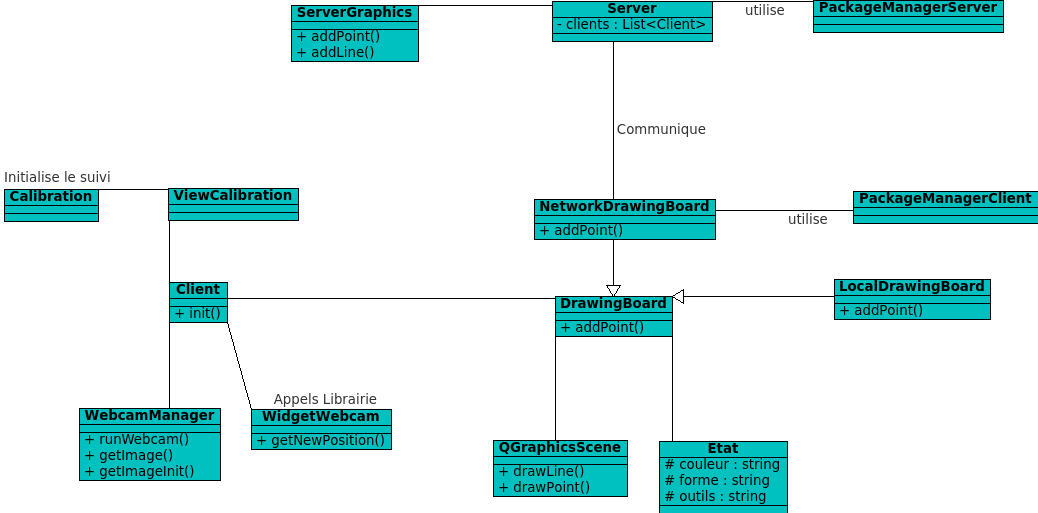
\includegraphics[scale=0.6]{../uml/classes.png}\\
						\caption{Diagramme de classe de l'application}
						\label{Diagramme de classe de l'application}
				\end{figure}

				
	
	\chapter{Réalisation}
		\section{Bibliothèque de suivi}
			Cette partie du développement a pour objectif de fournir un ensemble de fonctiionnalités permettant la reconnaissance et le suivi d'un objet, que nous appelerons ici Curseur, à partir d'images. \\
			L'objectif est de développer notre propre bibliothèque pour d'une part avoir un outil remplissant précisément nos objectifs et d'autre part de faire un travail de recherche et développement dans le domaine du traitement de l'image (en particulier le suivi d'objets). \\
			Un certain nombre de librairies existantes proposent des moyens nous facilitant la tâche, notamment grâce à des outils de reconnaissance de formes, de suivis de modèle ou d'évaluation de composantes connexes. 
			Le travail consiste donc à tirer partie de ces bibliothèques en les associant de manière à proposer des méthodes efficaces et simples à utiliser.
			Cela implique une bonne connaissance des outils existants, de leur compréhension et de leur utilisation conjointes dans le but de faire notre propre bibliothèque. \\
			La Bibliothèque de suivi sert à réaliser le suivi d'un objet, que nous appelerons ici Curseur, avec un minimum de connaissance en traitement des images.\\
			
					La bibliothèque fonctionne grâce à deux choses, une structure de données et deux fonctions enveloppe. \\
					Le curseur est représenté en mémoire sous la forme d'une strucure de données "Cursor". \\
					Cette structure de données est engendrée par la fonction "calibration" de la librairie, et est utilisée par la suite par l'autre fonction, la fonction "track", qui permet la mise à jour des informations relatives au curseur par rapport à une image.
					
				\newpage
				\subsubsection{Structure de données}
				\subsubsection{Fonctions}
			\subsection{}
		\section{Application}
	
	\chapter{Résultats}
		\section{Méthodes de suivi}
		\section{Application}
	
	\chapter{Conclusion}
		\section{Difficultés rencontrées}
		\section{Perspectives}
		\section{Conclusion}
	
	\chapter{Références}
	
	\part{Annexes}
	\appendix
		\chapter{Documentation de la librairie}	
\end{document}
